%Author Cesar
%Desc : For my presentations


\documentclass{beamer}\usetheme{Madrid} %

\setbeamercovered{invisible} % To remove the navigation symbols from
% the bottom of slides%
%\setbeamertemplate{navigation symbols}{}  %Disable the navigation
%

\usepackage{upquote} %proper quotation inside the verbatim

% sudo apt-get install texlive-full or texlive-science (the latter is minimal)
\usepackage{algorithmic}
\usepackage[spanish]{babel} 
\usepackage{algorithm2e}
\usepackage{color}
\usepackage{fancyvrb}

\usepackage{boxedminipage} %modified Madrid footer
\usepackage{graphicx}
\usepackage{caption}
\usepackage[utf8]{inputenc}
%\usepackage{bm}         % For typesetting bold math (not \mathbold)
%\logo{\includegraphics[height=0.6cm]{yourlogo.eps}}
%
\usepackage{amsmath}

\title[ACR]{Refinamiento Adaptivo de Código}
\author{C\'esar Sabater} \institute[UNR] {
%University of Strasbourg \\

\medskip
%{\emph{aravind.sukumaran-rajam@inria.fr}}\\
%\vspace{10px}
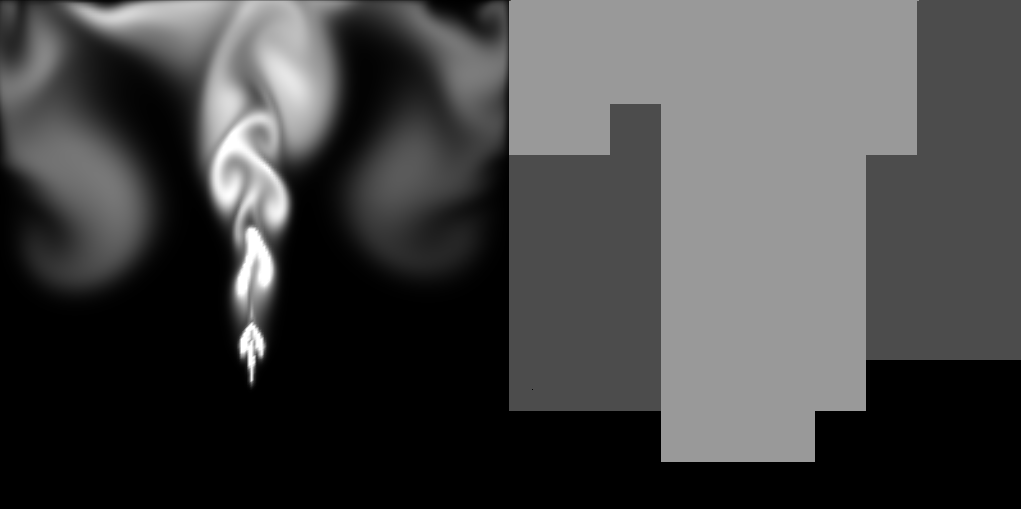
\includegraphics[scale=0.1]{img/logo.png} }

\subject{ Presentaci\'on Tesina 2017 } % \tiny{ }

\date{ \today} % \today will show
%current date.

\setbeamertemplate{navigation symbols}{}%remove navigation symbols 

%custom beaver footnote do what ever u want
\setbeamertemplate{footline} {%
\leavevmode
%
\hbox{%
\begin{beamercolorbox}[wd=.323\paperwidth,ht=2.25ex,dp=1ex,center]
    {author in head/foot}%
    \usebeamerfont{author in head/foot} Universidad Nacional de Rosario
\end{beamercolorbox}
%
\begin{beamercolorbox}[wd=.333\paperwidth,ht=2.25ex,dp=1ex,center]
    {title in head/foot}%
    \usebeamerfont{title in head/foot}\insertshorttitle
\end{beamercolorbox}
%
\begin{beamercolorbox}[wd=.3333\paperwidth,ht=2.25ex,dp=1ex,right]
    {date in head/foot}%
    \usebeamerfont{date in head/foot}\insertshortdate{}\hspace*{2em}
    \insertframenumber{} / \inserttotalframenumber\hspace*{1ex}
\end{beamercolorbox}
}%
\vskip0pt%
}

%\logo{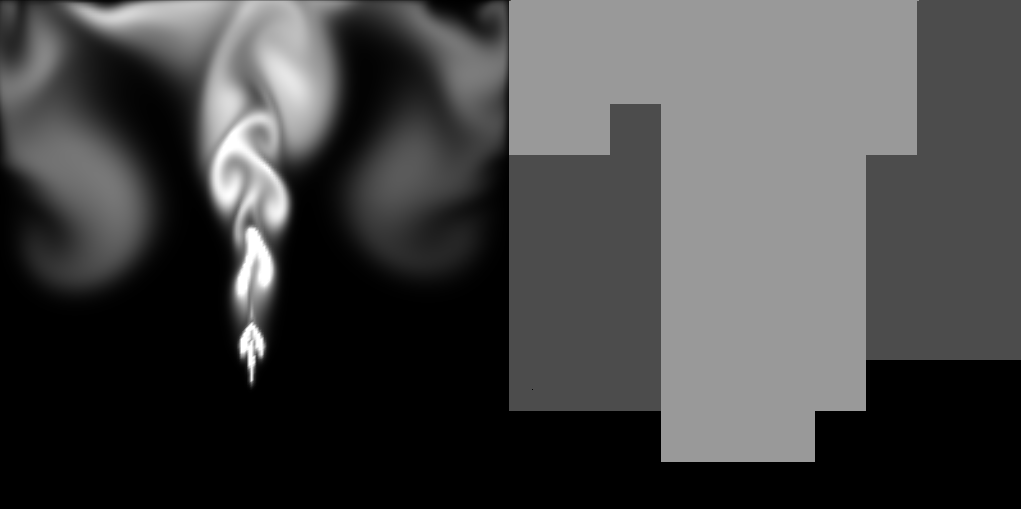
\includegraphics[scale=.04]{img/logo.png}}

\newcommand\codeHighlight[1]{\textcolor[rgb]{1,0,0}{\textbf{#1}}}

\newenvironment{rcases} {\left.
\begin{aligned}
    } {%
\end{aligned}
\right\rbrace}

\begin{document}
%
{ \setbeamertemplate{logo}{}
\begin{frame}
    \titlepage
    \vspace*{-25px}
    \begin{center}
        \large{ Presentaci\'on de Tesina }
    \end{center}
\end{frame}
}

%%%%%%%%%%%%%%%%%%%%%%%%%%%%%%%%%%%%%%%%%%%%%%%%%%%%%%%%%%%%%%%%%%%%%%%%%%%%%%%%
\begin{frame}
    \frametitle{Introduccion}
    %more concrete simualtions, but a more abstract kind of problem
    \begin{itemize}
    \item
    Muchas aplicaciones de \textbf{cómputo intensivo} realizan
    \textbf{cálculos aproximados}
    \item 
    Algunas Razones: 
    \begin{itemize}
        \item
			para simular objetos o fenomenos del mundo real
		\item
			trabajan con sensores limitados en precision
		\item
			estan sometidas a un deadline de tiempo
		\item
			calculan resultados preliminares
    \end{itemize}
    \end{itemize}
\end{frame}
%%%%%%%%%%%%%%%%%%%%%%%%%%%%%%%%%%%%%%%%%%%%%%%%%%%%%%%%%%%%%%%%%%%%%%%%%%%%%%%%
\begin{frame}
\frametitle{Introduccion}
Algunos ejemplos de estas aplicaciones son: 
    \begin{itemize}
        \item
			Simulaciónes Físicas
		\item
			Sensores de entrada, algoritmos de procesamiento
		\item
			Decodificación de Video en tiempo real
		\item 
			Predicción de Terremotos
		\item 
			Aplicaciones de exploracion de geofisica
    \end{itemize}
    %~ Generalmente, estas aplicaciones necesitan una gran cantitdad de poder computacional.
   %~ \begin{figure} 
	 %~ 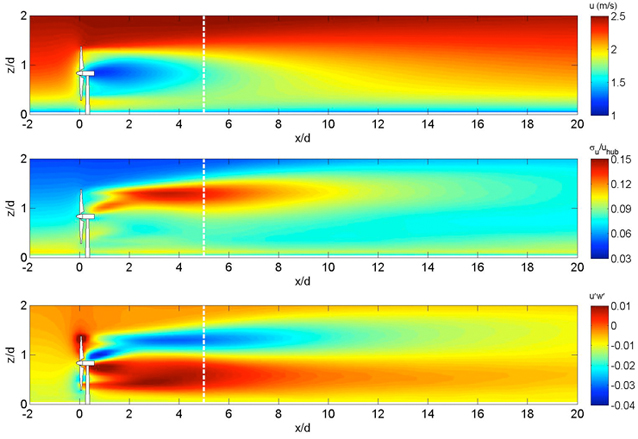
\includegraphics[scale=0.18]{img/wind_sim.jpg}
    %~ \end{figure}
\end{frame}
%%%%%%%%%%%%%%%%%%%%%%%%%%%%%%%%%%%%%%%%%%%%%%%%%%%%%%%%%%%%%%%%%%%%%%%%%%%%%%%%
\begin{frame}
\frametitle{Introduccion}
Normalmente, el desarrollo de estos 
algoritmos puede dividirse en \textbf{dos estapas}:
\begin{itemize}
\item Desarrollo de un kernel de computo ideal
	\begin{itemize} 
	\item ajuste del algoritmo
	\item debugueo
	\end{itemize}
\item Optimizacion a una version de produccion
	\begin{itemize}
	\item escalar al tamano real del problema
	\item satisfacer un deadline
	\end{itemize}
\end{itemize}
\end{frame}
%%%%%%%%%%%%%%%%%%%%%%%%%%%%%%%%%%%%%%%%%%%%%%%%%%%%%%%%%%%%%%%%%%%%%%%%%%%%%%%%
\begin{frame}
\frametitle{Introduccion}
Traducir un codigo ideal tiene complicaciones: 
\begin{itemize} 
\item es \textcolor{red}{complejo}
\item \textcolor{red}{lleva tiempo}
\item conduce a \textcolor{red}{codigos menos mantenibles}
\item hay que \textcolor{red}{hacerlo nuevamente} cuando hay cambios grandes en la estrategia
\end{itemize}
Esto se podria reducir con un \textbf{enfoque automatico de compilacion}
\end{frame}
%%%%%%%%%%%%%%%%%%%%%%%%%%%%%%%%%%%%%%%%%%%%%%%%%%%%%%%%%%%%%%%%%%%%%%%%%%%%%%%%
\begin{frame}
\frametitle{Introduccion}
Existen enfoques automaticos de optimizacion para computo intensivo:
\begin{itemize}
\item manteniendo la semantica original
\begin{itemize}
\item paralelizacion
\item localidad de datos
\item vectorizacion
\end{itemize}
\textcolor{blue}{bien abordados por los enfoques automaticos}
\item modificando la semantica original
\begin{itemize}
\item relajacion de dependencias
\item 


\end{itemize}




%~ %%%%%%%%%%%%%%%%%%%%%%%%%%%%%%%%%%%%%%%%%%%%%%%%%%%%%%%%%%%%%%t%%%%%%%%%%%%%%%%%%
%~ \begin{frame}
    %~ \frametitle{Ejemplo:  Simulación de Fluidos}
    %~ \begin{itemize}
        %~ \item
			%~ Calcula velocidad, presión, densidad, etc. de un en todo el espacio
			%~ que este ocupa a lo largo del tiempo.
		%~ \item
			%~ Las leyes que describen su evolución no tienen una
			%~ solucion  de forma cerrada.
		%~ \item 
			%~ Para algunas aplicaciónes, los estados necesitan ser calculados
			%~ con deadline de tiempo, como en la simulacion en tiempo real
    %~ \end{itemize}
    
   %~ \begin{figure} 
	  %~ 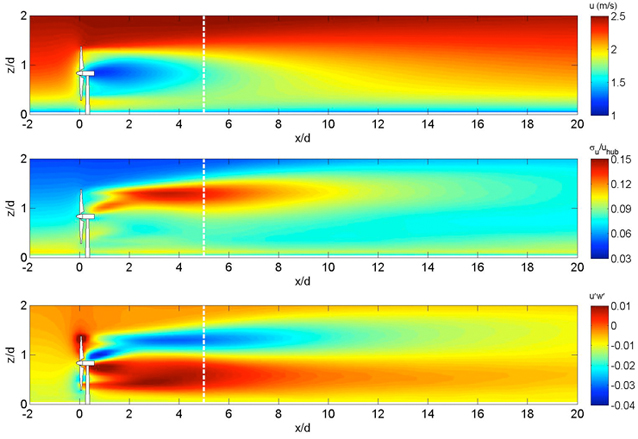
\includegraphics[scale=0.18]{img/wind_sim.jpg}
    %~ \end{figure}
%~ \end{frame}
%~ %%%%%%%%%%%%%%%%%%%%%%%%%%%%%%%%%%%%%%%%%%%%%%%%%%%%%%%%%%%%%%%%%%%%%%%%%%%%%%%%



% End of slides
\end{document}
 


